\documentclass[10pt]{article}

\usepackage[utf8x]{inputenc}
\usepackage[T1]{fontenc}
\usepackage[finnish]{babel}
\usepackage{amsmath}
\usepackage{amssymb}
\usepackage{amsfonts}
\usepackage{amsthm}
\usepackage{graphicx}
\usepackage[ruled]{algorithm2e}
\usepackage{empheq}
\usepackage{float}
\usepackage{graphicx}
\usepackage{color}

\title{Tietokantasovellus -- Dokumentaatio}
\date{2014, periodi 4}
\author{Rodion ``rodde'' Efremov}
\renewcommand*\rmdefault{iwona}
\definecolor{logobg}{RGB}{31,124,255}

\begin{document}

\pagenumbering{Roman}
\centerline{\colorbox{white}{\begin{minipage}{12cm}
\maketitle
\end{minipage}}}
\pagecolor{logobg}

\begin{center}
\centerline{
\includegraphics[width=450px, height=200px]{multilogo}}
\end{center}

\newpage
\pagecolor{white}
\tableofcontents
\newpage
\pagenumbering{arabic}

\section{Johdanto} Tämä dokumentti on tarkoitettu kuvaamaan Tietokantasovellus-kurssin (582203) aikana toteutettu verkkosovellus. Ajallisesti ottaen kurssisuoritukseni on ajoitettu kevään 2014 neljännelle periodille.

Toteutuskieleksi olen valinnut Javan (servletit Tomcat:n ajettavaksi), ja tietokannaksi olen valinnut niin ikään suositeltu PostgreSQL.

\section{Yleiskuva järjestelmästä (multilog)}
Aiheenani on keskustelufoorumin toteuttaminen. Järjestelmässä on kolme käyttäjäkategoriaa: 
\begin{itemize}
  \item ylläpitäjä (admin),
  \item moderaattori (moderator),
  \item käyttäjä (user).
\end{itemize}
Käyttäjä voi luoda tunnuksensa rekisteröitymällä sovellukseen. Ensimmäinen ylläpitäjä on luotu SQL-komennosta. Myöhemmin kun järjestelmässä alkaa olla käyttäjiä, ylläpitäjä voi ylentää tavallisen käyttäjän moderaattoriksi tai suoraan ylläpitäjäksi.Ylläpitäjä voi pudottaa moderaattorin peruskäyttäjäksi ja poistaa mielivaltaisen käyttäjän, jolloin myös moderaattoreiden poisto on mahdollista. Lisäksi, mikä tahansa rekisteröitynyt henkilö voi poistaa profiilinsa. Ylläpitäjä voi poistaa myös itsensä tai mielivaltaisen moderaattorin tai käyttäjän. Mitä tulee tilanteeseen, jossa ylläpitäjä poistaa itseään, onnistuu se vain jos poiston jälkeen järjestelmään jää vähintään yksi muu ylläpitäjä. (Järjestelmässä pitää olla vähintään yksi ylläpitäjä.) Moderaattori voi poistaa käyttäjien viestit, mikäli siihen on tarvetta. Lisäksi, moderaattori voi asettaa käyttäjät maksimissaan 7 vuorokauden käyttökieltoon. Toisaalta, moderaattori voi ylentää käyttäjän moderaattoriksi. Mitä tulee keskustelusäikeisiin, uusien luonti onnistuu jo peruskäyttäjän oikeuksilla; säikeiden poistaaminen vaatii vähintään moderaattorin oikeudet. Ylläpitäjät pystyvät tekemään samat toiminnot kuin moderaattoritkin. 

Mitä tulee itse foorumin rakenteeseen, alkusivulla voi selata ``teemoja''. Jokainen teema pitää sisällään vähintään yhden ``säikeen'', joista jälkimmäinen pitää sisällään siihen liittyvän keskusteluhistorian. Teemojen luonti ja poistaminen vaatii ylläpitäjän. Keskustelun lisäksi jokainen käyttäjä/moderaattori/ylläpitäjä voi lähettää yksityiset viestit mielivaltaiselle käyttäjälle ilman statusrajoja. Sovellus luo jokaiselle käyttäjälle profiilisivun, joissa näytetään (profiilin omistajan halutessa) sähköpostiosoite, syntymäpäivä, sukupuoli, oikea nimi. Profiilisivuilla esitetään aina avatar-kuva, lista postauksia ja postausten määrä.

Rekisteöityessään käyttäjä voi halutessaan lisätä avatar-kuvan, joka skaalataan tietynkokoiseksi; muussa tapauksessa käytetään oletus-avatar. Avatarkuvan voi lisätä/poistaa myös rekisteröitymisen jälkeen.

multilog sallii viesteissä erityistagien kirjoittamisen, joilla tekstiä pystyy muotoilemaan; alustavasti seuraavat muotoilut toteutetaan:
\begin{itemize}
  \item kursivointi,
  \item lihavointi,
  \item kiinteävälinen tekstitys (monospaced font),
  \item linkkien upottaminen,
  \item kuvien linkkittäminen tekstiin.
\end{itemize}

\section{Käyttötapaukset}
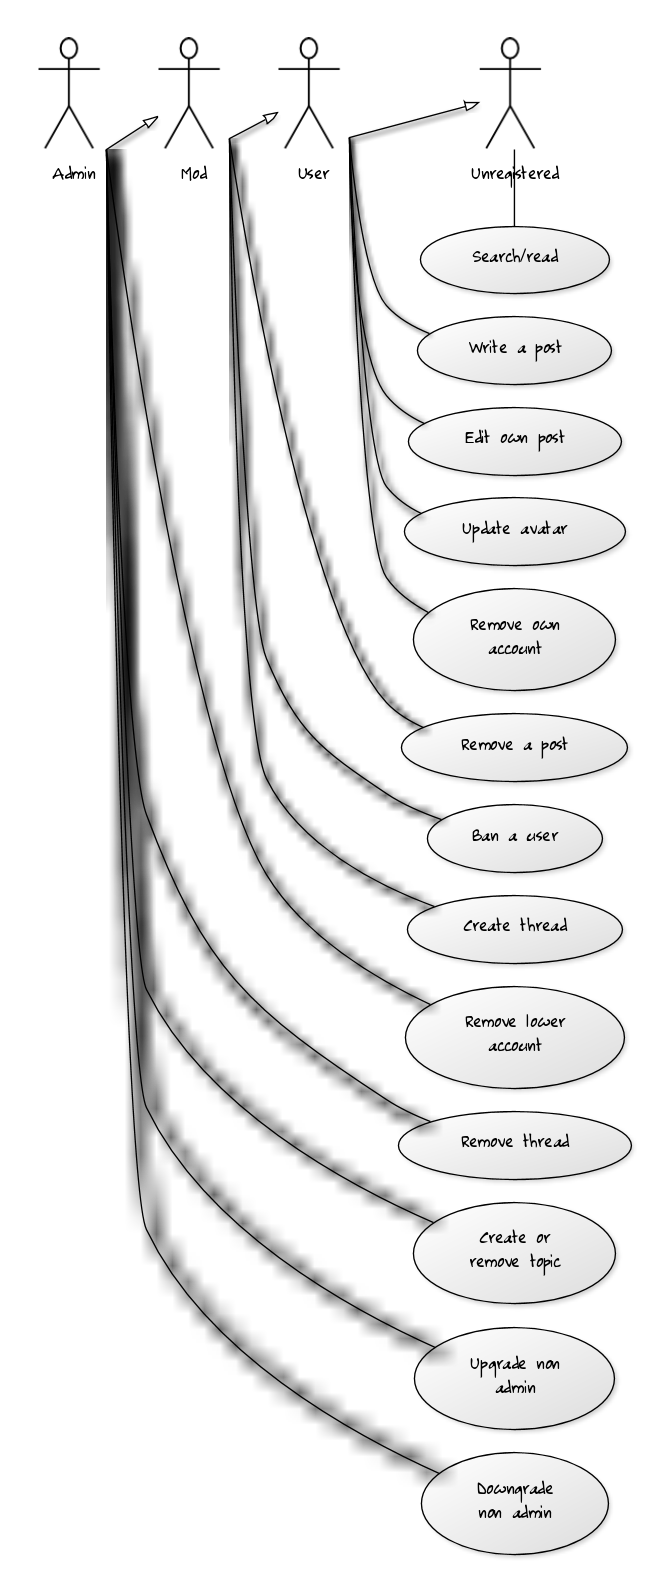
\includegraphics[width=\textwidth, height=\textheight, keepaspectratio]{multilog_use_case_diagram}
\newpage
\noindent Huomaa, että kaikki toiminnot paitsi lukeminen ja haku edellyttävät sisäänkirjautumisen.

\end{document}